\chapter{Evaluation of the Solution} % Main chapter title
\label{chap:solution_evaluation} 
After developing a new solution or project it is necessary to review if the final product has met the initial expectations. To accomplish this, the solution needs to be evaluated using a methodology that defines the system's functional and non-functional requirements. The designed model represents the ideal solution. The system is evaluated in several aspects of the dimensions, taking into account if the requirement was or not fulfilled, and with what quality.
\par
In this chapter, it will be presented the methodology that was used and how it was used.

\section{Evaluation Methodology}
\label{sec:evaluation_methodology}
To evaluate the quality of the solution, it was chosen to apply a \gls{QEF}. \gls{QEF} is used to identify the relevant quality factors to a certain business and to help on the definition of the metrics to objectively measure the quality factors that were identified \parencite{qef}. A model (available on appendix \ref{AppendixB}) was made to represent the ideal system. This model is divided into three different dimensions:  
\begin{itemize}
    \item Functional
    \item Security
    \item Efficiency
\end{itemize}

\par
The functional dimension is divided into two factors: the functional requirements and the user interaction. The first lists all needed use cases to be accomplished for the project to be a success. These will be measured by either the user has access to the functionality or not. In the case of FF11 and FF12, an intermediate point is acceptable, where it is available for just some of the actors. The second factor refers to the usability of the application. This will be measured mostly by questioning the users for their experience.
\par
The second dimension, security, refers to the concerns relatively to, as the name suggests, security of the platform. In this case, the only concerns that exist are associated to the security it, therefore it is its only factor. Similarly to the previous dimension, it will be measured by having or not fulfilled each of the requirements. There are intermediate positions for RN01 and RN02 when they are not put into practice every time.
\par
Lastly, the third dimension that will be evaluated is the efficiency. This dimension was split into two factors. The first concerns the overall structure of the page and the user can access its contents in an intuitive and direct way. The second one relates to the navigation resilience. In this factor, the requirements regarding the error handling and progress bars, showing progress for long tasks, will be evaluated. Both the factors of this dimension will be measured by having or not fulfilled the requirement. The only exception is the requirement EN02, where it is acceptable to have up to two long tasks not showing a progress bar.
\par
For this project to be successful, the quality factor in the \gls{QEF} should be above 90\% and have no dimension with a quality below 80\%. 


\section{Evaluation Results}
The model presented in section \ref{sec:evaluation_methodology} was applied to the final version of the prototype developed in the scope of this thesis. This version was finished in August \nth{6}, 2019 and the evaluation was made in September \nth{2}, 2019. 
\par
The requirements of the dimensions were weighted taking into account the priority and importance for the correct functioning of the platform, being 10 the most important and 2 the least important.
\par
The \textbf{functional dimension} is the biggest dimension since it contains all the use cases required by the platform. At this dimension there were three requirements that were postponed to a second version of the platform:

\begin{itemize}
    \item FF02 - Apply as a Service Provider
    \item FF03 - Apply as a Courier
    \item FF09 - Evaluate Experience
\end{itemize}

These requirements lost priority in comparison to others because in a first delivery, the prototype will run with a test service provider and limited number of couriers. The same happens for the FF09, where in a first phase, the experience will be reported directly to the existing service provider.
\par
This dimension was concluded with an estimated evaluation of 95.64\%.

\par

The second dimension, \textbf{security}, is one of the most important aspects in an e-commerce platform. It may attract or withdraw attention from possible customers and directly affects the reliability of the website. This dimension was completed in 100\%.

\par

Lastly, there is the \textbf{efficiency dimension}, which includes both the structure and navigation resilience. Since the platform still lacks beta testing in a real scenario (having real customers, couriers and service providers), there still room for improvement here. For this reason, the requirement \textit{EN03 - Application runtime does not have errors, and unexpected errors should be well treated} was only partially accomplished. With this, the evaluation result of this dimension was 83.33\%.

\par

Looking at the solution as a whole, the system had an evaluation of 95\%. This is a result that was better than expected. In the beginning of the project, the objective was to have a evaluation of at least 90\%. The system attained 5\% above than the required. It was also required to have no dimension with its evaluation below 80\%. As it was previously explained, the lowest score was 83\%.
\par
In the last page of the appendix \ref{AppendixB}, it is possible to check the evaluation matrix.

\section{Usability Surveys}
To understand how the platform meets the users needs, two surveys were run: one for the final customer perspective, and other for the service provider perspective. In the next sections, both surveys will be analyzed. 

\subsection{Customer Perspective Survey}
The first survey has as its purpose understand how the final customer feels about the usability of the SnapTasks portal. It includes a tutorial to place an order and explains how to use some of the  main features. In the appendix \ref{AppendixD} it is possible to check the original inquiry, and in the appendix \ref{AppendixF}, it is possible to consult the summary of the answers. This inquiry was made to seven people of different backgrounds.

\subsubsection{How do you rate the ease of registration and log in?}
This question has as its main purpose the evaluation of the log in and registration process. 
\par 
This question asks the user to evaluate in a scale of 1 to 5, where 1 is \textit{Very Hard} and 5 is \textit{Very Easy}. 
\par
This question had a result of \textbf{5}, out of 5. 


\subsubsection{How do you rate the presentation of service providers?}
This question has as its main purpose the evaluation of the home page, which is also the \gls{SPLP}. 
\par 
This question asks the user to evaluate in a scale of 1 to 5, where 1 is \textit{Very Hard to Understand} and 5 is \textit{Very Easy to Understand}. 
\par
This question had a result of \textbf{4.57}, out of 5. 

\subsubsection{How do you rate a service provider's presentation of services?}

This question has as its main purpose the evaluation of the \gls{SLP} of a given service provider and how those services are presented to the user. 
\par 
This question asks the user to evaluate in a scale of 1 to 5, where 1 is \textit{Very Hard to Understand} and 5 is \textit{Very Easy to Understand}. 
\par
This question had a result of \textbf{4.43}, out of 5. 

\subsubsection{Regarding the detail given on the page of a service, was the information sufficient?}

This question has as its main purpose the evaluation of the \gls{SDP} of a given service and how the details of a service are presented to the user. 
\par
This question asks the user to evaluate in a scale of 1 to 5, where 1 is \textit{Very Insufficient} and 5 is \textit{More than Sufficient}. 
\par
This question had a result of \textbf{4}, out of 5. 

\subsubsection{Was the price of a given service clear to you?}

This question has as its main purpose the evaluation of how clear the price of a given service was to the user.
\par
This question asks the user to evaluate in a scale of 1 to 5, where 1 is \textit{Not clear at all} and 5 is \textit{Very clear}. 
\par
This question had a result of \textbf{4.71}, out of 5. 

\subsubsection{How do you rate the ease of placing an order?}

This question has as its main purpose the evaluation the order placing and checkout experience. 
\par
This question asks the user to evaluate in a scale of 1 to 5, where 1 is \textit{Very hard} and 5 is \textit{Very easy}. 
\par
This question had a result of \textbf{4.86}, out of 5. 

\subsubsection{Was the data presented about the order placed (after purchase) clear?}

This question has as its main purpose the evaluation the order details page. 
\par 
This question asks the user to evaluate in a scale of 1 to 5, where 1 is \textit{Not clear at all} and 5 is \textit{Very clear}. 
\par
This question had a result of \textbf{4.86}, out of 5.

\subsubsection{How do you rate the information given in the order history?}

This question has as its main purpose the evaluation of the order history page and how the order history is presented to the user. 
\par
This question asks the user to evaluate in a scale of 1 to 5, where 1 is \textit{Very Insufficient} and 5 is \textit{More than Sufficient}. 
\par
This question had a result of \textbf{4.29}, out of 5. 

\subsubsection{Summary}
In this survey, the results of all questions were above 4, which is an excellent result. The graph in the figure \ref{fig:CustomerSurveyResults} presents a summary of the acquired results.


\begin{figure}[ht]
\centering
 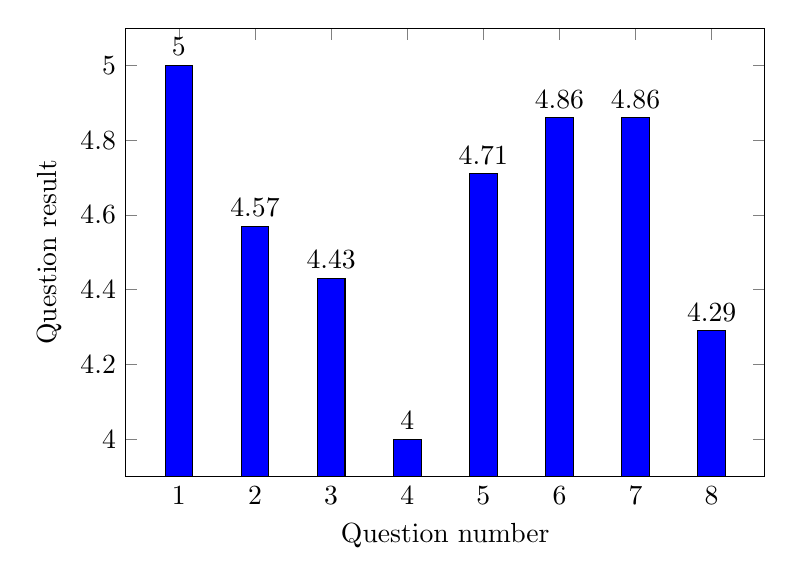
\begin{tikzpicture}
        \begin{axis}[
            symbolic x coords={1, 2, 3, 4, 5, 6, 7, 8},
            ylabel=Question result,
            xlabel=Question number,
            width=0.8\textwidth,
            height=0.6\textwidth,
            nodes near coords,
            nodes near coords align={vertical},
          ]
            \addplot[ybar,fill=blue] coordinates {
                (1,  5)
                (2,  4.57)
                (3,  4.43)
                (4,  4)
                (5,  4.71)
                (6,  4.86)
                (7,  4.86)
                (8,  4.29)
            };
        \end{axis}
    \end{tikzpicture}
\caption{Summary of results of the Customer Perspective Survey}
\label{fig:CustomerSurveyResults}
\end{figure}


\subsection{Service Provider Perspective Survey}
The second survey has as its purpose understand how service provider feels about the usability of the SnapTasks BackOffice Management app. It includes a tutorial of how to use some of the  main features. In the appendix \ref{AppendixE} it is possible to check the original inquiry, and in the appendix \ref{AppendixG}, it is possible to consult the summary of the answers. This inquiry was made to five people that work in service provision business.

\subsubsection{How do you rate the ease of log in?}
This question has as its main purpose the evaluation of the log in process. 
\par 
This question asks the user to evaluate in a scale of 1 to 5, where 1 is \textit{Very Hard} and 5 is \textit{Very Easy}. 
\par
This question had a result of \textbf{4.4}, out of 5. 

\subsubsection{How do you rate the presentation of service providers?}
This question has as its main purpose the evaluation of the presentation of the several service providers.
\par 
This question asks the user to evaluate in a scale of 1 to 5, where 1 is \textit{Very hard to understand} and 5 is \textit{Very easy to understand}. 
\par
This question had a result of \textbf{4}, out of 5. 

\subsubsection{How do you rate a service provider's presentation of services?}

This question has as its main purpose the evaluation of the presentation of the services of a given service provider.
\par 
This question asks the user to evaluate in a scale of 1 to 5, where 1 is \textit{Very hard to understand} and 5 is \textit{Very easy to understand}. 
\par
This question had a result of \textbf{4}, out of 5. 

\subsubsection{Regarding the detail given on the page of a service provider, was the information sufficient?}

This question has as its main purpose the evaluation of the presentation of the information regarding a given service provider. This information includes name, address, representatives and services.
\par 
This question asks the user to evaluate in a scale of 1 to 5, where 1 is \textit{Very insufficient} and 5 is \textit{More than sufficient}. 
\par
This question had a result of \textbf{3.6}, out of 5. 

\subsubsection{How do you rate the ease of updating the price of a service?}

This question has as its main purpose the evaluation of the process of price update on a given service.
\par 
This question asks the user to evaluate in a scale of 1 to 5, where 1 is \textit{Very insufficient} and 5 is \textit{More than sufficient}. 
\par
This question had a result of \textbf{3.2}, out of 5. 

\subsubsection{Was the presentation of the service data clear?}

This question has as its main purpose the evaluation of the presentation of details of a given service.
\par 
This question asks the user to evaluate in a scale of 1 to 5, where 1 is \textit{Not clear at all} and 5 is \textit{Very clear}. 
\par
This question had a result of \textbf{4}, out of 5. 

\subsubsection{Was the price presentation clear?}

This question has as its main purpose the evaluation of how clear the price presentation was to the user.
\par 
This question asks the user to evaluate in a scale of 1 to 5, where 1 is \textit{Not clear at all} and 5 is \textit{Very clear}. 
\par
This question had a result of \textbf{4.2}, out of 5.

\subsubsection{How do you rate the information given in the order history?}

This question has as its main purpose the evaluation of how clear the information present in the order history was.
\par 
This question asks the user to evaluate in a scale of 1 to 5, where 1 is \textit{Not clear at all} and 5 is \textit{Very clear}. 
\par
This question had a result of \textbf{4}, out of 5.

\subsubsection{How do you rate the information given in the details of an order (click "Details")?}

This question has as its main purpose the evaluation of how clear the information present in the order details was.
\par 
This question asks the user to evaluate in a scale of 1 to 5, where 1 is \textit{Not clear at all} and 5 is \textit{Very clear}. 
\par
This question had a result of \textbf{4}, out of 5.

\subsubsection{How do you rate the ease of changing an order status?}

This question has as its main purpose the evaluation of how easy it was to change the order status.
\par 
This question asks the user to evaluate in a scale of 1 to 5, where 1 is \textit{Very hard} and 5 is \textit{Very easy}. 
\par
This question had a result of \textbf{3.6}, out of 5.

\subsubsection{Summary}
In this survey, the results of all questions were above 3, which is an good result, despite being lower than the customer result. The graph in the figure \ref{fig:CustomerSurveyResults} presents a summary of the acquired results.


\begin{figure}[!ht]
\centering
 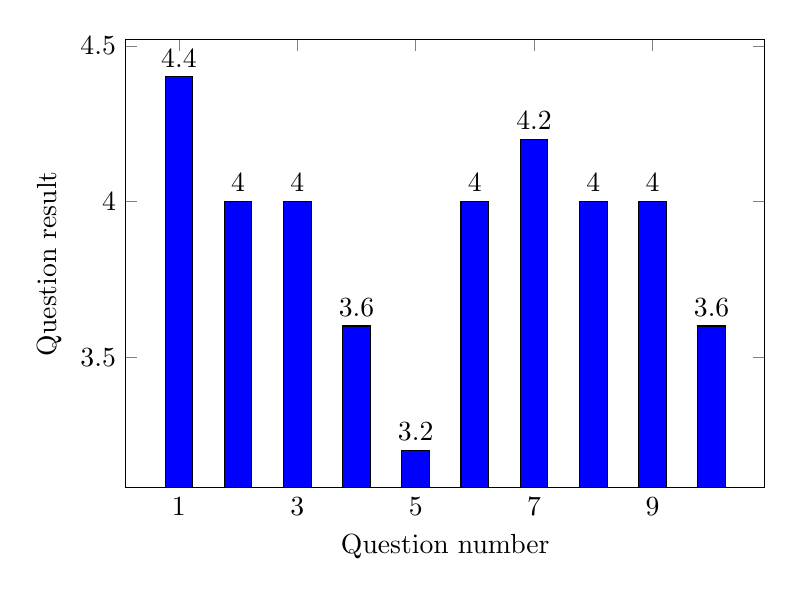
\begin{tikzpicture}
        \begin{axis}[
            symbolic x coords={1, 2, 3, 4, 5, 6, 7, 8, 9, 10},
            ylabel=Question result,
            xlabel=Question number,
            width=0.8\textwidth,
            height=0.6\textwidth,
            nodes near coords,
            nodes near coords align={vertical},
          ]
            \addplot[ybar,fill=blue] coordinates {
                (1,  4.4)
                (2,  4)
                (3,  4)
                (4,  3.6)
                (5,  3.2)
                (6,  4)
                (7,  4.2)
                (8,  4)
                (9,  4)
                (10, 3.6)
            };
        \end{axis}
    \end{tikzpicture}
\caption{Summary of results of the Customer Perspective Survey}
\label{fig:ServiceProviderSurveyResults}
\end{figure}
\pagebreak
\subsection{Results}
The results of both inquiries help us understand the points that should be improved in the future. There is room for improvement specially in the SnapTasks BackOffice Management app. Nevertheless, the results of both surveys were good, since all results were above 3 and taking into account that we are analysing the \gls{MVP} of the platform.
\par
In the SnapTasks portal (Customer Perspective Survey), the results were even better, having all results above 4, proving that the customers are already used to these type of platforms and could easily start using them for service provision.


